\documentclass[twoside]{book}

% Packages required by doxygen
\usepackage{fixltx2e}
\usepackage{calc}
\usepackage{doxygen}
\usepackage[export]{adjustbox} % also loads graphicx
\usepackage{graphicx}
\usepackage[utf8]{inputenc}
\usepackage{makeidx}
\usepackage{multicol}
\usepackage{multirow}
\PassOptionsToPackage{warn}{textcomp}
\usepackage{textcomp}
\usepackage[nointegrals]{wasysym}
\usepackage[table]{xcolor}

% Font selection
\usepackage[T1]{fontenc}
\usepackage[scaled=.90]{helvet}
\usepackage{courier}
\usepackage{amssymb}
\usepackage{sectsty}
\renewcommand{\familydefault}{\sfdefault}
\allsectionsfont{%
  \fontseries{bc}\selectfont%
  \color{darkgray}%
}
\renewcommand{\DoxyLabelFont}{%
  \fontseries{bc}\selectfont%
  \color{darkgray}%
}
\newcommand{\+}{\discretionary{\mbox{\scriptsize$\hookleftarrow$}}{}{}}

% Page & text layout
\usepackage{geometry}
\geometry{%
  a4paper,%
  top=2.5cm,%
  bottom=2.5cm,%
  left=2.5cm,%
  right=2.5cm%
}
\tolerance=750
\hfuzz=15pt
\hbadness=750
\setlength{\emergencystretch}{15pt}
\setlength{\parindent}{0cm}
\setlength{\parskip}{3ex plus 2ex minus 2ex}
\makeatletter
\renewcommand{\paragraph}{%
  \@startsection{paragraph}{4}{0ex}{-1.0ex}{1.0ex}{%
    \normalfont\normalsize\bfseries\SS@parafont%
  }%
}
\renewcommand{\subparagraph}{%
  \@startsection{subparagraph}{5}{0ex}{-1.0ex}{1.0ex}{%
    \normalfont\normalsize\bfseries\SS@subparafont%
  }%
}
\makeatother

% Headers & footers
\usepackage{fancyhdr}
\pagestyle{fancyplain}
\fancyhead[LE]{\fancyplain{}{\bfseries\thepage}}
\fancyhead[CE]{\fancyplain{}{}}
\fancyhead[RE]{\fancyplain{}{\bfseries\leftmark}}
\fancyhead[LO]{\fancyplain{}{\bfseries\rightmark}}
\fancyhead[CO]{\fancyplain{}{}}
\fancyhead[RO]{\fancyplain{}{\bfseries\thepage}}
\fancyfoot[LE]{\fancyplain{}{}}
\fancyfoot[CE]{\fancyplain{}{}}
\fancyfoot[RE]{\fancyplain{}{\bfseries\scriptsize Generated by Doxygen }}
\fancyfoot[LO]{\fancyplain{}{\bfseries\scriptsize Generated by Doxygen }}
\fancyfoot[CO]{\fancyplain{}{}}
\fancyfoot[RO]{\fancyplain{}{}}
\renewcommand{\footrulewidth}{0.4pt}
\renewcommand{\chaptermark}[1]{%
  \markboth{#1}{}%
}
\renewcommand{\sectionmark}[1]{%
  \markright{\thesection\ #1}%
}

% Indices & bibliography
\usepackage{natbib}
\usepackage[titles]{tocloft}
\setcounter{tocdepth}{3}
\setcounter{secnumdepth}{5}
\makeindex

% Hyperlinks (required, but should be loaded last)
\usepackage{ifpdf}
\ifpdf
  \usepackage[pdftex,pagebackref=true]{hyperref}
\else
  \usepackage[ps2pdf,pagebackref=true]{hyperref}
\fi
\hypersetup{%
  colorlinks=true,%
  linkcolor=blue,%
  citecolor=blue,%
  unicode%
}

% Custom commands
\newcommand{\clearemptydoublepage}{%
  \newpage{\pagestyle{empty}\cleardoublepage}%
}

\usepackage{caption}
\captionsetup{labelsep=space,justification=centering,font={bf},singlelinecheck=off,skip=4pt,position=top}

%===== C O N T E N T S =====

\begin{document}

% Titlepage & ToC
\hypersetup{pageanchor=false,
             bookmarksnumbered=true,
             pdfencoding=unicode
            }
\pagenumbering{alph}
\begin{titlepage}
\vspace*{7cm}
\begin{center}%
{\Large My Project }\\
\vspace*{1cm}
{\large Generated by Doxygen 1.8.13}\\
\end{center}
\end{titlepage}
\clearemptydoublepage
\pagenumbering{roman}
\tableofcontents
\clearemptydoublepage
\pagenumbering{arabic}
\hypersetup{pageanchor=true}

%--- Begin generated contents ---
\chapter{Hierarchical Index}
\section{Class Hierarchy}
This inheritance list is sorted roughly, but not completely, alphabetically\+:\begin{DoxyCompactList}
\item \contentsline{section}{com.\+fware.\+cspdt.\+cspm.\+editor.\+config.\+Csp\+M\+Color\+Constants}{\pageref{enumcom_1_1fware_1_1cspdt_1_1cspm_1_1editor_1_1config_1_1_csp_m_color_constants}}{}
\item \contentsline{section}{com.\+fware.\+cspdt.\+cspm.\+editor.\+config.\+Csp\+M\+Color\+Manager}{\pageref{classcom_1_1fware_1_1cspdt_1_1cspm_1_1editor_1_1config_1_1_csp_m_color_manager}}{}
\item \contentsline{section}{com.\+fware.\+cspdt.\+cspm.\+editor.\+preferences.\+Csp\+M\+Editor\+Preference\+Constants}{\pageref{interfacecom_1_1fware_1_1cspdt_1_1cspm_1_1editor_1_1preferences_1_1_csp_m_editor_preference_constants}}{}
\item \contentsline{section}{com.\+fware.\+cspdt.\+cspm.\+editor.\+project.\+Csp\+M\+Project}{\pageref{classcom_1_1fware_1_1cspdt_1_1cspm_1_1editor_1_1project_1_1_csp_m_project}}{}
\item \contentsline{section}{com.\+fware.\+cspdt.\+cspm.\+editor.\+project.\+Csp\+M\+Project\+Properties}{\pageref{classcom_1_1fware_1_1cspdt_1_1cspm_1_1editor_1_1project_1_1_csp_m_project_properties}}{}
\item \contentsline{section}{com.\+fware.\+cspdt.\+cspm.\+editor.\+config.\+Keywords}{\pageref{enumcom_1_1fware_1_1cspdt_1_1cspm_1_1editor_1_1config_1_1_keywords}}{}
\item Abstract\+Preference\+Initializer\begin{DoxyCompactList}
\item \contentsline{section}{com.\+fware.\+cspdt.\+cspm.\+editor.\+preferences.\+Csp\+M\+Editor\+Preference\+Initializer}{\pageref{classcom_1_1fware_1_1cspdt_1_1cspm_1_1editor_1_1preferences_1_1_csp_m_editor_preference_initializer}}{}
\end{DoxyCompactList}
\item Abstract\+U\+I\+Plugin\begin{DoxyCompactList}
\item \contentsline{section}{com.\+fware.\+cspdt.\+cspm.\+editor.\+Csp\+M\+Editor\+Plugin}{\pageref{classcom_1_1fware_1_1cspdt_1_1cspm_1_1editor_1_1_csp_m_editor_plugin}}{}
\end{DoxyCompactList}
\item Content\+Outline\+Page\begin{DoxyCompactList}
\item \contentsline{section}{com.\+fware.\+cspdt.\+cspm.\+editor.\+outline.\+Csp\+M\+Content\+Outline\+Page}{\pageref{classcom_1_1fware_1_1cspdt_1_1cspm_1_1editor_1_1outline_1_1_csp_m_content_outline_page}}{}
\end{DoxyCompactList}
\item Csp\+Analyser\+Listener\begin{DoxyCompactList}
\item \contentsline{section}{com.\+fware.\+cspdt.\+cspm.\+editor.\+marker.\+Csp\+M\+Marking\+Error\+Handler}{\pageref{classcom_1_1fware_1_1cspdt_1_1cspm_1_1editor_1_1marker_1_1_csp_m_marking_error_handler}}{}
\end{DoxyCompactList}
\item Default\+Hyperlink\+Presenter\begin{DoxyCompactList}
\item \contentsline{section}{com.\+fware.\+cspdt.\+cspm.\+editor.\+link.\+Csp\+M\+Hyperlink\+Presenter}{\pageref{classcom_1_1fware_1_1cspdt_1_1cspm_1_1editor_1_1link_1_1_csp_m_hyperlink_presenter}}{}
\end{DoxyCompactList}
\item Default\+Indent\+Line\+Auto\+Edit\+Strategy\begin{DoxyCompactList}
\item \contentsline{section}{com.\+fware.\+cspdt.\+cspm.\+editor.\+config.\+Csp\+M\+Auto\+Indent\+Strategy}{\pageref{classcom_1_1fware_1_1cspdt_1_1cspm_1_1editor_1_1config_1_1_csp_m_auto_indent_strategy}}{}
\end{DoxyCompactList}
\item Extended\+Depth\+First\+Adapter\begin{DoxyCompactList}
\item \contentsline{section}{com.\+fware.\+cspdt.\+cspm.\+editor.\+link.\+Csp\+M\+Ref\+Extractor}{\pageref{classcom_1_1fware_1_1cspdt_1_1cspm_1_1editor_1_1link_1_1_csp_m_ref_extractor}}{}
\item \contentsline{section}{com.\+fware.\+cspdt.\+cspm.\+editor.\+outline.\+Csp\+M\+Ast\+Tree\+Node\+Generator}{\pageref{classcom_1_1fware_1_1cspdt_1_1cspm_1_1editor_1_1outline_1_1_csp_m_ast_tree_node_generator}}{}
\end{DoxyCompactList}
\item Fast\+Partitioner\begin{DoxyCompactList}
\item \contentsline{section}{com.\+fware.\+cspdt.\+cspm.\+editor.\+partition.\+Csp\+M\+Partitioner}{\pageref{classcom_1_1fware_1_1cspdt_1_1cspm_1_1editor_1_1partition_1_1_csp_m_partitioner}}{}
\end{DoxyCompactList}
\item Field\+Editor\+Preference\+Page\begin{DoxyCompactList}
\item \contentsline{section}{com.\+fware.\+cspdt.\+cspm.\+editor.\+preferences.\+Csp\+M\+Editor\+Preference\+Page}{\pageref{classcom_1_1fware_1_1cspdt_1_1cspm_1_1editor_1_1preferences_1_1_csp_m_editor_preference_page}}{}
\end{DoxyCompactList}
\item File\+Document\+Provider\begin{DoxyCompactList}
\item \contentsline{section}{com.\+fware.\+cspdt.\+cspm.\+editor.\+Csp\+M\+Document\+Provider}{\pageref{classcom_1_1fware_1_1cspdt_1_1cspm_1_1editor_1_1_csp_m_document_provider}}{}
\end{DoxyCompactList}
\item I\+Content\+Assist\+Processor\begin{DoxyCompactList}
\item \contentsline{section}{com.\+fware.\+cspdt.\+cspm.\+editor.\+config.\+Csp\+M\+Process\+Completion\+Processor}{\pageref{classcom_1_1fware_1_1cspdt_1_1cspm_1_1editor_1_1config_1_1_csp_m_process_completion_processor}}{}
\end{DoxyCompactList}
\item I\+Editor\+Part\begin{DoxyCompactList}
\item \contentsline{section}{com.\+fware.\+cspdt.\+cspm.\+editor.\+Csp\+M\+Editor}{\pageref{classcom_1_1fware_1_1cspdt_1_1cspm_1_1editor_1_1_csp_m_editor}}{}
\end{DoxyCompactList}
\item I\+Executable\+Extension\begin{DoxyCompactList}
\item \contentsline{section}{com.\+fware.\+cspdt.\+cspm.\+editor.\+wizards.\+Csp\+M\+New\+Project\+Wizard}{\pageref{classcom_1_1fware_1_1cspdt_1_1cspm_1_1editor_1_1wizards_1_1_csp_m_new_project_wizard}}{}
\end{DoxyCompactList}
\item I\+Hyperlink\begin{DoxyCompactList}
\item \contentsline{section}{com.\+fware.\+cspdt.\+cspm.\+editor.\+link.\+Csp\+M\+Hyperlink}{\pageref{classcom_1_1fware_1_1cspdt_1_1cspm_1_1editor_1_1link_1_1_csp_m_hyperlink}}{}
\end{DoxyCompactList}
\item I\+Hyperlink\+Detector\begin{DoxyCompactList}
\item \contentsline{section}{com.\+fware.\+cspdt.\+cspm.\+editor.\+link.\+Csp\+M\+Hyperlink\+Detector}{\pageref{classcom_1_1fware_1_1cspdt_1_1cspm_1_1editor_1_1link_1_1_csp_m_hyperlink_detector}}{}
\end{DoxyCompactList}
\item I\+New\+Wizard\begin{DoxyCompactList}
\item \contentsline{section}{com.\+fware.\+cspdt.\+cspm.\+editor.\+wizards.\+Csp\+M\+New\+File\+Wizard}{\pageref{classcom_1_1fware_1_1cspdt_1_1cspm_1_1editor_1_1wizards_1_1_csp_m_new_file_wizard}}{}
\item \contentsline{section}{com.\+fware.\+cspdt.\+cspm.\+editor.\+wizards.\+Csp\+M\+New\+Project\+Wizard}{\pageref{classcom_1_1fware_1_1cspdt_1_1cspm_1_1editor_1_1wizards_1_1_csp_m_new_project_wizard}}{}
\end{DoxyCompactList}
\item I\+Predicate\+Rule\begin{DoxyCompactList}
\item \contentsline{section}{com.\+fware.\+cspdt.\+cspm.\+editor.\+partition.\+Process\+Rule}{\pageref{classcom_1_1fware_1_1cspdt_1_1cspm_1_1editor_1_1partition_1_1_process_rule}}{}
\end{DoxyCompactList}
\item I\+Presentation\+Damager\begin{DoxyCompactList}
\item \contentsline{section}{com.\+fware.\+cspdt.\+cspm.\+editor.\+config.\+Non\+Rule\+Based\+Damager\+Repairer}{\pageref{classcom_1_1fware_1_1cspdt_1_1cspm_1_1editor_1_1config_1_1_non_rule_based_damager_repairer}}{}
\end{DoxyCompactList}
\item I\+Presentation\+Repairer\begin{DoxyCompactList}
\item \contentsline{section}{com.\+fware.\+cspdt.\+cspm.\+editor.\+config.\+Non\+Rule\+Based\+Damager\+Repairer}{\pageref{classcom_1_1fware_1_1cspdt_1_1cspm_1_1editor_1_1config_1_1_non_rule_based_damager_repairer}}{}
\end{DoxyCompactList}
\item I\+Reconciling\+Strategy\begin{DoxyCompactList}
\item \contentsline{section}{com.\+fware.\+cspdt.\+cspm.\+editor.\+config.\+Csp\+M\+Reconciling\+Strategy}{\pageref{classcom_1_1fware_1_1cspdt_1_1cspm_1_1editor_1_1config_1_1_csp_m_reconciling_strategy}}{}
\end{DoxyCompactList}
\item I\+Runnable\+With\+Progress\begin{DoxyCompactList}
\item \contentsline{section}{com.\+fware.\+cspdt.\+cspm.\+editor.\+wizards.\+Csp\+M\+New\+Project\+Operation}{\pageref{classcom_1_1fware_1_1cspdt_1_1cspm_1_1editor_1_1wizards_1_1_csp_m_new_project_operation}}{}
\end{DoxyCompactList}
\item I\+Text\+Double\+Click\+Strategy\begin{DoxyCompactList}
\item \contentsline{section}{com.\+fware.\+cspdt.\+cspm.\+editor.\+config.\+Csp\+M\+Double\+Click\+Strategy}{\pageref{classcom_1_1fware_1_1cspdt_1_1cspm_1_1editor_1_1config_1_1_csp_m_double_click_strategy}}{}
\end{DoxyCompactList}
\item I\+Text\+Hover\begin{DoxyCompactList}
\item \contentsline{section}{com.\+fware.\+cspdt.\+cspm.\+editor.\+hover.\+Csp\+M\+Text\+Hover}{\pageref{classcom_1_1fware_1_1cspdt_1_1cspm_1_1editor_1_1hover_1_1_csp_m_text_hover}}{}
\end{DoxyCompactList}
\item I\+Whitespace\+Detector\begin{DoxyCompactList}
\item \contentsline{section}{com.\+fware.\+cspdt.\+cspm.\+editor.\+scanner.\+Csp\+Whitespace\+Detector}{\pageref{classcom_1_1fware_1_1cspdt_1_1cspm_1_1editor_1_1scanner_1_1_csp_whitespace_detector}}{}
\end{DoxyCompactList}
\item I\+Word\+Detector\begin{DoxyCompactList}
\item \contentsline{section}{com.\+fware.\+cspdt.\+cspm.\+editor.\+scanner.\+Csp\+M\+Keyword\+Detector}{\pageref{classcom_1_1fware_1_1cspdt_1_1cspm_1_1editor_1_1scanner_1_1_csp_m_keyword_detector}}{}
\item \contentsline{section}{com.\+fware.\+cspdt.\+cspm.\+editor.\+scanner.\+Csp\+M\+Name\+Detector}{\pageref{classcom_1_1fware_1_1cspdt_1_1cspm_1_1editor_1_1scanner_1_1_csp_m_name_detector}}{}
\end{DoxyCompactList}
\item I\+Workbench\+Preference\+Page\begin{DoxyCompactList}
\item \contentsline{section}{com.\+fware.\+cspdt.\+cspm.\+editor.\+preferences.\+Csp\+M\+Editor\+Preference\+Page}{\pageref{classcom_1_1fware_1_1cspdt_1_1cspm_1_1editor_1_1preferences_1_1_csp_m_editor_preference_page}}{}
\end{DoxyCompactList}
\item Rule\+Based\+Partition\+Scanner\begin{DoxyCompactList}
\item \contentsline{section}{com.\+fware.\+cspdt.\+cspm.\+editor.\+partition.\+Csp\+M\+Partition\+Scanner}{\pageref{classcom_1_1fware_1_1cspdt_1_1cspm_1_1editor_1_1partition_1_1_csp_m_partition_scanner}}{}
\end{DoxyCompactList}
\item Rule\+Based\+Scanner\begin{DoxyCompactList}
\item \contentsline{section}{com.\+fware.\+cspdt.\+cspm.\+editor.\+scanner.\+Csp\+M\+Scanner}{\pageref{classcom_1_1fware_1_1cspdt_1_1cspm_1_1editor_1_1scanner_1_1_csp_m_scanner}}{}
\end{DoxyCompactList}
\item Text\+Editor\begin{DoxyCompactList}
\item \contentsline{section}{com.\+fware.\+cspdt.\+cspm.\+editor.\+Csp\+M\+Editor}{\pageref{classcom_1_1fware_1_1cspdt_1_1cspm_1_1editor_1_1_csp_m_editor}}{}
\end{DoxyCompactList}
\item Text\+Editor\+Action\+Contributor\begin{DoxyCompactList}
\item \contentsline{section}{com.\+fware.\+cspdt.\+cspm.\+editor.\+Csp\+M\+File\+Editor\+Contributor}{\pageref{classcom_1_1fware_1_1cspdt_1_1cspm_1_1editor_1_1_csp_m_file_editor_contributor}}{}
\end{DoxyCompactList}
\item Text\+Source\+Viewer\+Configuration\begin{DoxyCompactList}
\item \contentsline{section}{com.\+fware.\+cspdt.\+cspm.\+editor.\+config.\+Csp\+M\+Source\+Viewer\+Configuration}{\pageref{classcom_1_1fware_1_1cspdt_1_1cspm_1_1editor_1_1config_1_1_csp_m_source_viewer_configuration}}{}
\end{DoxyCompactList}
\item Tree\+Node\begin{DoxyCompactList}
\item \contentsline{section}{com.\+fware.\+cspdt.\+cspm.\+editor.\+outline.\+Csp\+M\+Outline\+Tree\+Node}{\pageref{classcom_1_1fware_1_1cspdt_1_1cspm_1_1editor_1_1outline_1_1_csp_m_outline_tree_node}}{}
\end{DoxyCompactList}
\item Tree\+Node\+Content\+Provider\begin{DoxyCompactList}
\item \contentsline{section}{com.\+fware.\+cspdt.\+cspm.\+editor.\+outline.\+Csp\+M\+Outline\+Content\+Provider}{\pageref{classcom_1_1fware_1_1cspdt_1_1cspm_1_1editor_1_1outline_1_1_csp_m_outline_content_provider}}{}
\end{DoxyCompactList}
\item Wizard\begin{DoxyCompactList}
\item \contentsline{section}{com.\+fware.\+cspdt.\+cspm.\+editor.\+wizards.\+Csp\+M\+New\+File\+Wizard}{\pageref{classcom_1_1fware_1_1cspdt_1_1cspm_1_1editor_1_1wizards_1_1_csp_m_new_file_wizard}}{}
\item \contentsline{section}{com.\+fware.\+cspdt.\+cspm.\+editor.\+wizards.\+Csp\+M\+New\+Project\+Wizard}{\pageref{classcom_1_1fware_1_1cspdt_1_1cspm_1_1editor_1_1wizards_1_1_csp_m_new_project_wizard}}{}
\end{DoxyCompactList}
\item Wizard\+Page\begin{DoxyCompactList}
\item \contentsline{section}{com.\+fware.\+cspdt.\+cspm.\+editor.\+wizards.\+Csp\+M\+New\+File\+Wizard\+Page}{\pageref{classcom_1_1fware_1_1cspdt_1_1cspm_1_1editor_1_1wizards_1_1_csp_m_new_file_wizard_page}}{}
\end{DoxyCompactList}
\end{DoxyCompactList}

\chapter{Class Index}
\section{Class List}
Here are the classes, structs, unions and interfaces with brief descriptions\+:\begin{DoxyCompactList}
\item\contentsline{section}{\hyperlink{classcom_1_1fware_1_1cspdt_1_1cspm_1_1core_1_1parser_1_1_csp_m_analyser_exception}{com.\+fware.\+cspdt.\+cspm.\+core.\+parser.\+Csp\+M\+Analyser\+Exception} \\*Excecao disparada quando a analise lexica de um no na ast falha }{\pageref{classcom_1_1fware_1_1cspdt_1_1cspm_1_1core_1_1parser_1_1_csp_m_analyser_exception}}{}
\item\contentsline{section}{\hyperlink{classcom_1_1fware_1_1cspdt_1_1cspm_1_1core_1_1_csp_m_core_plugin}{com.\+fware.\+cspdt.\+cspm.\+core.\+Csp\+M\+Core\+Plugin} \\*Classe principal do plug-\/in }{\pageref{classcom_1_1fware_1_1cspdt_1_1cspm_1_1core_1_1_csp_m_core_plugin}}{}
\item\contentsline{section}{\hyperlink{classcom_1_1fware_1_1cspdt_1_1cspm_1_1core_1_1model_1_1_csp_m_model}{com.\+fware.\+cspdt.\+cspm.\+core.\+model.\+Csp\+M\+Model} \\*Essa classe contera os dados de analise do codigo }{\pageref{classcom_1_1fware_1_1cspdt_1_1cspm_1_1core_1_1model_1_1_csp_m_model}}{}
\item\contentsline{section}{\hyperlink{classcom_1_1fware_1_1cspdt_1_1cspm_1_1core_1_1parser_1_1_csp_m_parser}{com.\+fware.\+cspdt.\+cspm.\+core.\+parser.\+Csp\+M\+Parser} \\*Uma classe para usar a analise lexica e sintatica do codigo C\+SP }{\pageref{classcom_1_1fware_1_1cspdt_1_1cspm_1_1core_1_1parser_1_1_csp_m_parser}}{}
\item\contentsline{section}{\hyperlink{classcom_1_1fware_1_1cspdt_1_1cspm_1_1core_1_1parser_1_1_csp_m_parser_exception}{com.\+fware.\+cspdt.\+cspm.\+core.\+parser.\+Csp\+M\+Parser\+Exception} \\*Excecao disparada quando a analise sintatica de um no na ast falha }{\pageref{classcom_1_1fware_1_1cspdt_1_1cspm_1_1core_1_1parser_1_1_csp_m_parser_exception}}{}
\item\contentsline{section}{\hyperlink{classcom_1_1fware_1_1cspdt_1_1cspm_1_1core_1_1model_1_1_csp_m_ref}{com.\+fware.\+cspdt.\+cspm.\+core.\+model.\+Csp\+M\+Ref} \\*Essa classe representa uma referencia dentro do documento C\+SP }{\pageref{classcom_1_1fware_1_1cspdt_1_1cspm_1_1core_1_1model_1_1_csp_m_ref}}{}
\item\contentsline{section}{\hyperlink{classcom_1_1fware_1_1cspdt_1_1cspm_1_1core_1_1model_1_1_token_extractor}{com.\+fware.\+cspdt.\+cspm.\+core.\+model.\+Token\+Extractor} \\*Classe que extrai tokens da ast }{\pageref{classcom_1_1fware_1_1cspdt_1_1cspm_1_1core_1_1model_1_1_token_extractor}}{}
\end{DoxyCompactList}

\chapter{Class Documentation}
\hypertarget{classcom_1_1fware_1_1cspdt_1_1cspm_1_1core_1_1parser_1_1_csp_m_analyser_exception}{}\section{com.\+fware.\+cspdt.\+cspm.\+core.\+parser.\+Csp\+M\+Analyser\+Exception Class Reference}
\label{classcom_1_1fware_1_1cspdt_1_1cspm_1_1core_1_1parser_1_1_csp_m_analyser_exception}\index{com.\+fware.\+cspdt.\+cspm.\+core.\+parser.\+Csp\+M\+Analyser\+Exception@{com.\+fware.\+cspdt.\+cspm.\+core.\+parser.\+Csp\+M\+Analyser\+Exception}}


Excecao disparada quando a analise lexica de um no na ast falha.  


Inheritance diagram for com.\+fware.\+cspdt.\+cspm.\+core.\+parser.\+Csp\+M\+Analyser\+Exception\+:\begin{figure}[H]
\begin{center}
\leavevmode
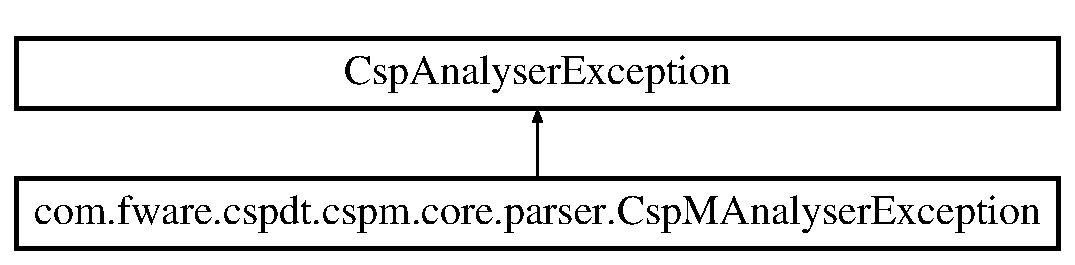
\includegraphics[height=2.000000cm]{classcom_1_1fware_1_1cspdt_1_1cspm_1_1core_1_1parser_1_1_csp_m_analyser_exception}
\end{center}
\end{figure}
\subsection*{Public Member Functions}
\begin{DoxyCompactItemize}
\item 
\hyperlink{classcom_1_1fware_1_1cspdt_1_1cspm_1_1core_1_1parser_1_1_csp_m_analyser_exception_a4223ce06d5b1dedd5b60bf823488c7cf}{Csp\+M\+Analyser\+Exception} (String msg, Node node)
\begin{DoxyCompactList}\small\item\em Contrutor Padrao. \end{DoxyCompactList}\end{DoxyCompactItemize}


\subsection{Detailed Description}
Excecao disparada quando a analise lexica de um no na ast falha. 

\begin{DoxyAuthor}{Author}
A\+L\+V\+A\+RO, E\+V\+E\+R\+A\+L\+DA, F\+E\+L\+I\+PE, J\+O\+N\+A\+T\+H\+AN, J\+U\+V\+E\+N\+AL 
\end{DoxyAuthor}


\subsection{Constructor \& Destructor Documentation}
\mbox{\Hypertarget{classcom_1_1fware_1_1cspdt_1_1cspm_1_1core_1_1parser_1_1_csp_m_analyser_exception_a4223ce06d5b1dedd5b60bf823488c7cf}\label{classcom_1_1fware_1_1cspdt_1_1cspm_1_1core_1_1parser_1_1_csp_m_analyser_exception_a4223ce06d5b1dedd5b60bf823488c7cf}} 
\index{com\+::fware\+::cspdt\+::cspm\+::core\+::parser\+::\+Csp\+M\+Analyser\+Exception@{com\+::fware\+::cspdt\+::cspm\+::core\+::parser\+::\+Csp\+M\+Analyser\+Exception}!Csp\+M\+Analyser\+Exception@{Csp\+M\+Analyser\+Exception}}
\index{Csp\+M\+Analyser\+Exception@{Csp\+M\+Analyser\+Exception}!com\+::fware\+::cspdt\+::cspm\+::core\+::parser\+::\+Csp\+M\+Analyser\+Exception@{com\+::fware\+::cspdt\+::cspm\+::core\+::parser\+::\+Csp\+M\+Analyser\+Exception}}
\subsubsection{\texorpdfstring{Csp\+M\+Analyser\+Exception()}{CspMAnalyserException()}}
{\footnotesize\ttfamily com.\+fware.\+cspdt.\+cspm.\+core.\+parser.\+Csp\+M\+Analyser\+Exception.\+Csp\+M\+Analyser\+Exception (\begin{DoxyParamCaption}\item[{String}]{msg,  }\item[{Node}]{node }\end{DoxyParamCaption})\hspace{0.3cm}{\ttfamily [inline]}}



Contrutor Padrao. 


\begin{DoxyParams}{Parameters}
{\em msg} & A mensagem de erro \\
\hline
{\em node} & O no onde foi encontrado o erro \\
\hline
\end{DoxyParams}


The documentation for this class was generated from the following file\+:\begin{DoxyCompactItemize}
\item 
C\+:/\+Users/\+E\+V\+A/\+Downloads/eclipse/workspace/cspdt/com.\+fware.\+cspdt.\+cspm.\+core/src/com/fware/cspdt/cspm/core/parser/Csp\+M\+Analyser\+Exception.\+java\end{DoxyCompactItemize}

\hypertarget{classcom_1_1fware_1_1cspdt_1_1cspm_1_1core_1_1_csp_m_core_plugin}{}\section{com.\+fware.\+cspdt.\+cspm.\+core.\+Csp\+M\+Core\+Plugin Class Reference}
\label{classcom_1_1fware_1_1cspdt_1_1cspm_1_1core_1_1_csp_m_core_plugin}\index{com.\+fware.\+cspdt.\+cspm.\+core.\+Csp\+M\+Core\+Plugin@{com.\+fware.\+cspdt.\+cspm.\+core.\+Csp\+M\+Core\+Plugin}}


Classe principal do plug-\/in.  


Inheritance diagram for com.\+fware.\+cspdt.\+cspm.\+core.\+Csp\+M\+Core\+Plugin\+:\begin{figure}[H]
\begin{center}
\leavevmode
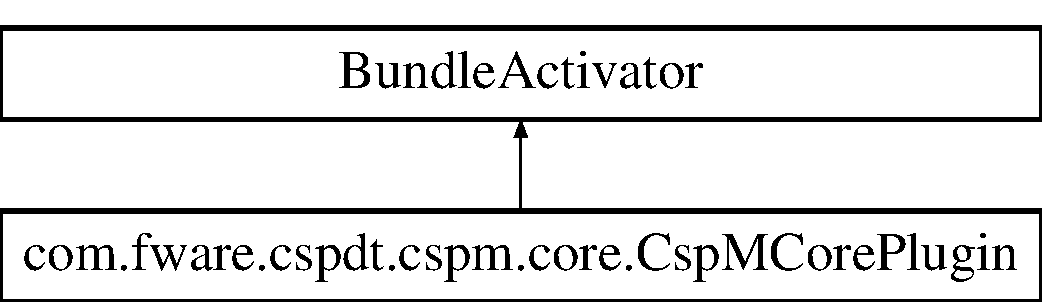
\includegraphics[height=2.000000cm]{classcom_1_1fware_1_1cspdt_1_1cspm_1_1core_1_1_csp_m_core_plugin}
\end{center}
\end{figure}
\subsection*{Public Member Functions}
\begin{DoxyCompactItemize}
\item 
\mbox{\Hypertarget{classcom_1_1fware_1_1cspdt_1_1cspm_1_1core_1_1_csp_m_core_plugin_a1d041e63450748ffe936d4e41b3de5aa}\label{classcom_1_1fware_1_1cspdt_1_1cspm_1_1core_1_1_csp_m_core_plugin_a1d041e63450748ffe936d4e41b3de5aa}} 
void {\bfseries start} (Bundle\+Context bundle\+Context)  throws Exception 
\item 
\mbox{\Hypertarget{classcom_1_1fware_1_1cspdt_1_1cspm_1_1core_1_1_csp_m_core_plugin_aa11fe9ba973ee978252af28e5e16b605}\label{classcom_1_1fware_1_1cspdt_1_1cspm_1_1core_1_1_csp_m_core_plugin_aa11fe9ba973ee978252af28e5e16b605}} 
void {\bfseries stop} (Bundle\+Context bundle\+Context)  throws Exception 
\end{DoxyCompactItemize}


\subsection{Detailed Description}
Classe principal do plug-\/in. 

Contem o contexto que comunica com o Eclipse.

\begin{DoxyAuthor}{Author}
A\+L\+V\+A\+RO, E\+V\+E\+R\+A\+L\+DA, F\+E\+L\+I\+PE, J\+O\+N\+A\+T\+H\+AN, J\+U\+V\+E\+N\+AL 
\end{DoxyAuthor}


The documentation for this class was generated from the following file\+:\begin{DoxyCompactItemize}
\item 
C\+:/\+Users/\+E\+V\+A/\+Downloads/eclipse/workspace/cspdt/com.\+fware.\+cspdt.\+cspm.\+core/src/com/fware/cspdt/cspm/core/Csp\+M\+Core\+Plugin.\+java\end{DoxyCompactItemize}

\hypertarget{classcom_1_1fware_1_1cspdt_1_1cspm_1_1core_1_1model_1_1_csp_m_model}{}\section{com.\+fware.\+cspdt.\+cspm.\+core.\+model.\+Csp\+M\+Model Class Reference}
\label{classcom_1_1fware_1_1cspdt_1_1cspm_1_1core_1_1model_1_1_csp_m_model}\index{com.\+fware.\+cspdt.\+cspm.\+core.\+model.\+Csp\+M\+Model@{com.\+fware.\+cspdt.\+cspm.\+core.\+model.\+Csp\+M\+Model}}


Essa classe contera os dados de analise do codigo.  


\subsection*{Public Member Functions}
\begin{DoxyCompactItemize}
\item 
\mbox{\Hypertarget{classcom_1_1fware_1_1cspdt_1_1cspm_1_1core_1_1model_1_1_csp_m_model_a35c09e3b9d951b0c6cfbdda824f53c2f}\label{classcom_1_1fware_1_1cspdt_1_1cspm_1_1core_1_1model_1_1_csp_m_model_a35c09e3b9d951b0c6cfbdda824f53c2f}} 
{\bfseries Csp\+M\+Model} (I\+File \hyperlink{classcom_1_1fware_1_1cspdt_1_1cspm_1_1core_1_1model_1_1_csp_m_model_ade0ba2ecf90a09b10dda2370389c41ef}{file})
\end{DoxyCompactItemize}
\subsection*{Public Attributes}
\begin{DoxyCompactItemize}
\item 
\mbox{\Hypertarget{classcom_1_1fware_1_1cspdt_1_1cspm_1_1core_1_1model_1_1_csp_m_model_ade0ba2ecf90a09b10dda2370389c41ef}\label{classcom_1_1fware_1_1cspdt_1_1cspm_1_1core_1_1model_1_1_csp_m_model_ade0ba2ecf90a09b10dda2370389c41ef}} 
I\+File \hyperlink{classcom_1_1fware_1_1cspdt_1_1cspm_1_1core_1_1model_1_1_csp_m_model_ade0ba2ecf90a09b10dda2370389c41ef}{file}
\begin{DoxyCompactList}\small\item\em Faz referencia ao arquivo onde se encontra o codigo C\+SP. \end{DoxyCompactList}\item 
\mbox{\Hypertarget{classcom_1_1fware_1_1cspdt_1_1cspm_1_1core_1_1model_1_1_csp_m_model_a542b3eb8b7b6ac41151f05c512e7be55}\label{classcom_1_1fware_1_1cspdt_1_1cspm_1_1core_1_1model_1_1_csp_m_model_a542b3eb8b7b6ac41151f05c512e7be55}} 
Start \hyperlink{classcom_1_1fware_1_1cspdt_1_1cspm_1_1core_1_1model_1_1_csp_m_model_a542b3eb8b7b6ac41151f05c512e7be55}{ast}
\begin{DoxyCompactList}\small\item\em Arvore sintatica (A\+ST) da linguagem C\+SP. \end{DoxyCompactList}\item 
\mbox{\Hypertarget{classcom_1_1fware_1_1cspdt_1_1cspm_1_1core_1_1model_1_1_csp_m_model_a1ed92caf2e91df005219ad24bce038a5}\label{classcom_1_1fware_1_1cspdt_1_1cspm_1_1core_1_1model_1_1_csp_m_model_a1ed92caf2e91df005219ad24bce038a5}} 
final Linked\+List$<$ \hyperlink{classcom_1_1fware_1_1cspdt_1_1cspm_1_1core_1_1model_1_1_csp_m_ref}{Csp\+M\+Ref} $>$ \hyperlink{classcom_1_1fware_1_1cspdt_1_1cspm_1_1core_1_1model_1_1_csp_m_model_a1ed92caf2e91df005219ad24bce038a5}{toc\+Refs} = new Linked\+List$<$\hyperlink{classcom_1_1fware_1_1cspdt_1_1cspm_1_1core_1_1model_1_1_csp_m_ref}{Csp\+M\+Ref}$>$()
\begin{DoxyCompactList}\small\item\em Conjunto de referencias do modelo para o outline. \end{DoxyCompactList}\item 
\mbox{\Hypertarget{classcom_1_1fware_1_1cspdt_1_1cspm_1_1core_1_1model_1_1_csp_m_model_a2c0b1dcabb33ffd380f10fb11306dd82}\label{classcom_1_1fware_1_1cspdt_1_1cspm_1_1core_1_1model_1_1_csp_m_model_a2c0b1dcabb33ffd380f10fb11306dd82}} 
final Linked\+List$<$ \hyperlink{classcom_1_1fware_1_1cspdt_1_1cspm_1_1core_1_1model_1_1_csp_m_ref}{Csp\+M\+Ref} $>$ \hyperlink{classcom_1_1fware_1_1cspdt_1_1cspm_1_1core_1_1model_1_1_csp_m_model_a2c0b1dcabb33ffd380f10fb11306dd82}{channel\+Refs} = new Linked\+List$<$\hyperlink{classcom_1_1fware_1_1cspdt_1_1cspm_1_1core_1_1model_1_1_csp_m_ref}{Csp\+M\+Ref}$>$()
\begin{DoxyCompactList}\small\item\em Conjunto de referencias de canais do C\+SP. \end{DoxyCompactList}\item 
\mbox{\Hypertarget{classcom_1_1fware_1_1cspdt_1_1cspm_1_1core_1_1model_1_1_csp_m_model_a11cbd033d64ecbce9f28fcc2854ff9cc}\label{classcom_1_1fware_1_1cspdt_1_1cspm_1_1core_1_1model_1_1_csp_m_model_a11cbd033d64ecbce9f28fcc2854ff9cc}} 
final Linked\+List$<$ \hyperlink{classcom_1_1fware_1_1cspdt_1_1cspm_1_1core_1_1model_1_1_csp_m_ref}{Csp\+M\+Ref} $>$ \hyperlink{classcom_1_1fware_1_1cspdt_1_1cspm_1_1core_1_1model_1_1_csp_m_model_a11cbd033d64ecbce9f28fcc2854ff9cc}{function\+Refs} = new Linked\+List$<$\hyperlink{classcom_1_1fware_1_1cspdt_1_1cspm_1_1core_1_1model_1_1_csp_m_ref}{Csp\+M\+Ref}$>$()
\begin{DoxyCompactList}\small\item\em Conjunto de referencias de funcoes do C\+SP. \end{DoxyCompactList}\item 
\mbox{\Hypertarget{classcom_1_1fware_1_1cspdt_1_1cspm_1_1core_1_1model_1_1_csp_m_model_a8d7c1a9c9b394f2ff289027785731191}\label{classcom_1_1fware_1_1cspdt_1_1cspm_1_1core_1_1model_1_1_csp_m_model_a8d7c1a9c9b394f2ff289027785731191}} 
final Linked\+List$<$ \hyperlink{classcom_1_1fware_1_1cspdt_1_1cspm_1_1core_1_1model_1_1_csp_m_ref}{Csp\+M\+Ref} $>$ \hyperlink{classcom_1_1fware_1_1cspdt_1_1cspm_1_1core_1_1model_1_1_csp_m_model_a8d7c1a9c9b394f2ff289027785731191}{process\+Refs} = new Linked\+List$<$\hyperlink{classcom_1_1fware_1_1cspdt_1_1cspm_1_1core_1_1model_1_1_csp_m_ref}{Csp\+M\+Ref}$>$()
\begin{DoxyCompactList}\small\item\em Conjunto de referencias de processos do C\+SP. \end{DoxyCompactList}\item 
\mbox{\Hypertarget{classcom_1_1fware_1_1cspdt_1_1cspm_1_1core_1_1model_1_1_csp_m_model_acc4e8a009ea0daa5ccbd3752d3e6b89f}\label{classcom_1_1fware_1_1cspdt_1_1cspm_1_1core_1_1model_1_1_csp_m_model_acc4e8a009ea0daa5ccbd3752d3e6b89f}} 
final Linked\+List$<$ \hyperlink{classcom_1_1fware_1_1cspdt_1_1cspm_1_1core_1_1model_1_1_csp_m_ref}{Csp\+M\+Ref} $>$ \hyperlink{classcom_1_1fware_1_1cspdt_1_1cspm_1_1core_1_1model_1_1_csp_m_model_acc4e8a009ea0daa5ccbd3752d3e6b89f}{constant\+Refs} = new Linked\+List$<$\hyperlink{classcom_1_1fware_1_1cspdt_1_1cspm_1_1core_1_1model_1_1_csp_m_ref}{Csp\+M\+Ref}$>$()
\begin{DoxyCompactList}\small\item\em Conjunto de referencias de constantes do C\+SP. \end{DoxyCompactList}\item 
\mbox{\Hypertarget{classcom_1_1fware_1_1cspdt_1_1cspm_1_1core_1_1model_1_1_csp_m_model_aef5c4cf5b8e4548181e5f8ba831086d2}\label{classcom_1_1fware_1_1cspdt_1_1cspm_1_1core_1_1model_1_1_csp_m_model_aef5c4cf5b8e4548181e5f8ba831086d2}} 
final Linked\+List$<$ \hyperlink{classcom_1_1fware_1_1cspdt_1_1cspm_1_1core_1_1model_1_1_csp_m_ref}{Csp\+M\+Ref} $>$ \hyperlink{classcom_1_1fware_1_1cspdt_1_1cspm_1_1core_1_1model_1_1_csp_m_model_aef5c4cf5b8e4548181e5f8ba831086d2}{datatype\+Refs} = new Linked\+List$<$\hyperlink{classcom_1_1fware_1_1cspdt_1_1cspm_1_1core_1_1model_1_1_csp_m_ref}{Csp\+M\+Ref}$>$()
\begin{DoxyCompactList}\small\item\em Conjunto de referencias de tipos de dados do C\+SP. \end{DoxyCompactList}\item 
\mbox{\Hypertarget{classcom_1_1fware_1_1cspdt_1_1cspm_1_1core_1_1model_1_1_csp_m_model_aa5ad45b134156a73c9a46408a74f7846}\label{classcom_1_1fware_1_1cspdt_1_1cspm_1_1core_1_1model_1_1_csp_m_model_aa5ad45b134156a73c9a46408a74f7846}} 
final Linked\+List$<$ \hyperlink{classcom_1_1fware_1_1cspdt_1_1cspm_1_1core_1_1model_1_1_csp_m_ref}{Csp\+M\+Ref} $>$ \hyperlink{classcom_1_1fware_1_1cspdt_1_1cspm_1_1core_1_1model_1_1_csp_m_model_aa5ad45b134156a73c9a46408a74f7846}{subtype\+Refs} = new Linked\+List$<$\hyperlink{classcom_1_1fware_1_1cspdt_1_1cspm_1_1core_1_1model_1_1_csp_m_ref}{Csp\+M\+Ref}$>$()
\begin{DoxyCompactList}\small\item\em Conjunto de referencias de subtipos de dados do C\+SP. \end{DoxyCompactList}\item 
\mbox{\Hypertarget{classcom_1_1fware_1_1cspdt_1_1cspm_1_1core_1_1model_1_1_csp_m_model_a56e20f5eedda41f95187c8b81506b7a5}\label{classcom_1_1fware_1_1cspdt_1_1cspm_1_1core_1_1model_1_1_csp_m_model_a56e20f5eedda41f95187c8b81506b7a5}} 
final Linked\+List$<$ \hyperlink{classcom_1_1fware_1_1cspdt_1_1cspm_1_1core_1_1model_1_1_csp_m_ref}{Csp\+M\+Ref} $>$ \hyperlink{classcom_1_1fware_1_1cspdt_1_1cspm_1_1core_1_1model_1_1_csp_m_model_a56e20f5eedda41f95187c8b81506b7a5}{nametype\+Refs} = new Linked\+List$<$\hyperlink{classcom_1_1fware_1_1cspdt_1_1cspm_1_1core_1_1model_1_1_csp_m_ref}{Csp\+M\+Ref}$>$()
\begin{DoxyCompactList}\small\item\em Conjunto de referencias de tipos nomeados do C\+SP. \end{DoxyCompactList}\item 
\mbox{\Hypertarget{classcom_1_1fware_1_1cspdt_1_1cspm_1_1core_1_1model_1_1_csp_m_model_a475286ab7d66ee1906b991fcbef7931a}\label{classcom_1_1fware_1_1cspdt_1_1cspm_1_1core_1_1model_1_1_csp_m_model_a475286ab7d66ee1906b991fcbef7931a}} 
final Linked\+List$<$ \hyperlink{classcom_1_1fware_1_1cspdt_1_1cspm_1_1core_1_1model_1_1_csp_m_ref}{Csp\+M\+Ref} $>$ \hyperlink{classcom_1_1fware_1_1cspdt_1_1cspm_1_1core_1_1model_1_1_csp_m_model_a475286ab7d66ee1906b991fcbef7931a}{abstract\+Refs} = new Linked\+List$<$\hyperlink{classcom_1_1fware_1_1cspdt_1_1cspm_1_1core_1_1model_1_1_csp_m_ref}{Csp\+M\+Ref}$>$()
\begin{DoxyCompactList}\small\item\em Conjunto de referencias de abstracoes do C\+SP. \end{DoxyCompactList}\item 
\mbox{\Hypertarget{classcom_1_1fware_1_1cspdt_1_1cspm_1_1core_1_1model_1_1_csp_m_model_ab7a908078c826ce8442303ff57b6fc69}\label{classcom_1_1fware_1_1cspdt_1_1cspm_1_1core_1_1model_1_1_csp_m_model_ab7a908078c826ce8442303ff57b6fc69}} 
final Map$<$ String, String $>$ \hyperlink{classcom_1_1fware_1_1cspdt_1_1cspm_1_1core_1_1model_1_1_csp_m_model_ab7a908078c826ce8442303ff57b6fc69}{channel\+Definitions} = new Hash\+Map$<$String, String$>$()
\begin{DoxyCompactList}\small\item\em Conjunto de definicoes de canais do C\+SP. \end{DoxyCompactList}\item 
\mbox{\Hypertarget{classcom_1_1fware_1_1cspdt_1_1cspm_1_1core_1_1model_1_1_csp_m_model_ab8fd2eeabc86c739674447223495266b}\label{classcom_1_1fware_1_1cspdt_1_1cspm_1_1core_1_1model_1_1_csp_m_model_ab8fd2eeabc86c739674447223495266b}} 
final Map$<$ String, String $>$ \hyperlink{classcom_1_1fware_1_1cspdt_1_1cspm_1_1core_1_1model_1_1_csp_m_model_ab8fd2eeabc86c739674447223495266b}{function\+Definitions} = new Hash\+Map$<$String, String$>$()
\begin{DoxyCompactList}\small\item\em Conjunto de definicoes de funcoes do C\+SP. \end{DoxyCompactList}\item 
\mbox{\Hypertarget{classcom_1_1fware_1_1cspdt_1_1cspm_1_1core_1_1model_1_1_csp_m_model_aed9a230ed281bd58e6d28a542bb5f01a}\label{classcom_1_1fware_1_1cspdt_1_1cspm_1_1core_1_1model_1_1_csp_m_model_aed9a230ed281bd58e6d28a542bb5f01a}} 
final Map$<$ String, String $>$ \hyperlink{classcom_1_1fware_1_1cspdt_1_1cspm_1_1core_1_1model_1_1_csp_m_model_aed9a230ed281bd58e6d28a542bb5f01a}{process\+Definitions} = new Hash\+Map$<$String, String$>$()
\begin{DoxyCompactList}\small\item\em Conjunto de definicoes de processos do C\+SP. \end{DoxyCompactList}\item 
\mbox{\Hypertarget{classcom_1_1fware_1_1cspdt_1_1cspm_1_1core_1_1model_1_1_csp_m_model_ab6b6af2200f818acba683e14e6014957}\label{classcom_1_1fware_1_1cspdt_1_1cspm_1_1core_1_1model_1_1_csp_m_model_ab6b6af2200f818acba683e14e6014957}} 
final Map$<$ String, String $>$ \hyperlink{classcom_1_1fware_1_1cspdt_1_1cspm_1_1core_1_1model_1_1_csp_m_model_ab6b6af2200f818acba683e14e6014957}{constant\+Definitions} = new Hash\+Map$<$String, String$>$()
\begin{DoxyCompactList}\small\item\em Conjunto de definicoes de constantes do C\+SP. \end{DoxyCompactList}\item 
\mbox{\Hypertarget{classcom_1_1fware_1_1cspdt_1_1cspm_1_1core_1_1model_1_1_csp_m_model_a925ce7d39dc1949824c100cd019fa3e9}\label{classcom_1_1fware_1_1cspdt_1_1cspm_1_1core_1_1model_1_1_csp_m_model_a925ce7d39dc1949824c100cd019fa3e9}} 
final Map$<$ String, String $>$ \hyperlink{classcom_1_1fware_1_1cspdt_1_1cspm_1_1core_1_1model_1_1_csp_m_model_a925ce7d39dc1949824c100cd019fa3e9}{datatype\+Definitions} = new Hash\+Map$<$String, String$>$()
\begin{DoxyCompactList}\small\item\em Conjunto de definicoes de tipos de dados do C\+SP. \end{DoxyCompactList}\item 
\mbox{\Hypertarget{classcom_1_1fware_1_1cspdt_1_1cspm_1_1core_1_1model_1_1_csp_m_model_a635d031bc7fefc435cc03539814a1fd2}\label{classcom_1_1fware_1_1cspdt_1_1cspm_1_1core_1_1model_1_1_csp_m_model_a635d031bc7fefc435cc03539814a1fd2}} 
final Map$<$ String, String $>$ \hyperlink{classcom_1_1fware_1_1cspdt_1_1cspm_1_1core_1_1model_1_1_csp_m_model_a635d031bc7fefc435cc03539814a1fd2}{subtype\+Definitions} = new Hash\+Map$<$String, String$>$()
\begin{DoxyCompactList}\small\item\em Conjunto de definicoes de subtipos de dados do C\+SP. \end{DoxyCompactList}\item 
\mbox{\Hypertarget{classcom_1_1fware_1_1cspdt_1_1cspm_1_1core_1_1model_1_1_csp_m_model_a16e2992fb47391708e35f7f054563764}\label{classcom_1_1fware_1_1cspdt_1_1cspm_1_1core_1_1model_1_1_csp_m_model_a16e2992fb47391708e35f7f054563764}} 
final Map$<$ String, String $>$ \hyperlink{classcom_1_1fware_1_1cspdt_1_1cspm_1_1core_1_1model_1_1_csp_m_model_a16e2992fb47391708e35f7f054563764}{nametype\+Definitions} = new Hash\+Map$<$String, String$>$()
\begin{DoxyCompactList}\small\item\em Conjunto de definicoes de tipos nomeados do C\+SP. \end{DoxyCompactList}\item 
\mbox{\Hypertarget{classcom_1_1fware_1_1cspdt_1_1cspm_1_1core_1_1model_1_1_csp_m_model_a846aaf42254ecf524887f5fcec29e2ac}\label{classcom_1_1fware_1_1cspdt_1_1cspm_1_1core_1_1model_1_1_csp_m_model_a846aaf42254ecf524887f5fcec29e2ac}} 
final Map$<$ String, String $>$ \hyperlink{classcom_1_1fware_1_1cspdt_1_1cspm_1_1core_1_1model_1_1_csp_m_model_a846aaf42254ecf524887f5fcec29e2ac}{abstract\+Definitions} = new Hash\+Map$<$String, String$>$()
\begin{DoxyCompactList}\small\item\em Conjunto de definicoes de abstracoes do C\+SP. \end{DoxyCompactList}\end{DoxyCompactItemize}


\subsection{Detailed Description}
Essa classe contera os dados de analise do codigo. 

A classe contem a ast do codigo e os conjuntos de funcoes, processos, tipos e outras caracteristicas da linguagem C\+SP

\begin{DoxyAuthor}{Author}
A\+L\+V\+A\+RO, E\+V\+E\+R\+A\+L\+DA, F\+E\+L\+I\+PE, J\+O\+N\+A\+T\+H\+AN, J\+U\+V\+E\+N\+AL 
\end{DoxyAuthor}


The documentation for this class was generated from the following file\+:\begin{DoxyCompactItemize}
\item 
C\+:/\+Users/\+E\+V\+A/\+Downloads/eclipse/workspace/cspdt/com.\+fware.\+cspdt.\+cspm.\+core/src/com/fware/cspdt/cspm/core/model/Csp\+M\+Model.\+java\end{DoxyCompactItemize}

\hypertarget{classcom_1_1fware_1_1cspdt_1_1cspm_1_1core_1_1parser_1_1_csp_m_parser}{}\section{com.\+fware.\+cspdt.\+cspm.\+core.\+parser.\+Csp\+M\+Parser Class Reference}
\label{classcom_1_1fware_1_1cspdt_1_1cspm_1_1core_1_1parser_1_1_csp_m_parser}\index{com.\+fware.\+cspdt.\+cspm.\+core.\+parser.\+Csp\+M\+Parser@{com.\+fware.\+cspdt.\+cspm.\+core.\+parser.\+Csp\+M\+Parser}}


Uma classe para usar a analise lexica e sintatica do codigo C\+SP.  


\subsection*{Public Member Functions}
\begin{DoxyCompactItemize}
\item 
\hyperlink{classcom_1_1fware_1_1cspdt_1_1cspm_1_1core_1_1model_1_1_csp_m_model}{Csp\+M\+Model} \hyperlink{classcom_1_1fware_1_1cspdt_1_1cspm_1_1core_1_1parser_1_1_csp_m_parser_abcd9ef2aecf9c7a1de12da310357e831}{get\+Info} (I\+File file, Csp\+Analyser\+Listener analyser)  throws Csp\+M\+Parser\+Exception, Csp\+Analyser\+Exception 
\begin{DoxyCompactList}\small\item\em Metodo para analise do codigo. \end{DoxyCompactList}\item 
\hyperlink{classcom_1_1fware_1_1cspdt_1_1cspm_1_1core_1_1model_1_1_csp_m_model}{Csp\+M\+Model} \hyperlink{classcom_1_1fware_1_1cspdt_1_1cspm_1_1core_1_1parser_1_1_csp_m_parser_a4fb399c8ac1c19c8b089f3021cf56986}{parse} (I\+File file, Csp\+Analyser\+Listener listener, boolean stop\+On\+Error, boolean debugging)
\begin{DoxyCompactList}\small\item\em Metodo para analise do arquivo. \end{DoxyCompactList}\end{DoxyCompactItemize}


\subsection{Detailed Description}
Uma classe para usar a analise lexica e sintatica do codigo C\+SP. 

\begin{DoxyAuthor}{Author}
A\+L\+V\+A\+RO, E\+V\+E\+R\+A\+L\+DA, F\+E\+L\+I\+PE, J\+O\+N\+A\+T\+H\+AN, J\+U\+V\+E\+N\+AL 
\end{DoxyAuthor}


\subsection{Member Function Documentation}
\mbox{\Hypertarget{classcom_1_1fware_1_1cspdt_1_1cspm_1_1core_1_1parser_1_1_csp_m_parser_abcd9ef2aecf9c7a1de12da310357e831}\label{classcom_1_1fware_1_1cspdt_1_1cspm_1_1core_1_1parser_1_1_csp_m_parser_abcd9ef2aecf9c7a1de12da310357e831}} 
\index{com\+::fware\+::cspdt\+::cspm\+::core\+::parser\+::\+Csp\+M\+Parser@{com\+::fware\+::cspdt\+::cspm\+::core\+::parser\+::\+Csp\+M\+Parser}!get\+Info@{get\+Info}}
\index{get\+Info@{get\+Info}!com\+::fware\+::cspdt\+::cspm\+::core\+::parser\+::\+Csp\+M\+Parser@{com\+::fware\+::cspdt\+::cspm\+::core\+::parser\+::\+Csp\+M\+Parser}}
\subsubsection{\texorpdfstring{get\+Info()}{getInfo()}}
{\footnotesize\ttfamily \hyperlink{classcom_1_1fware_1_1cspdt_1_1cspm_1_1core_1_1model_1_1_csp_m_model}{Csp\+M\+Model} com.\+fware.\+cspdt.\+cspm.\+core.\+parser.\+Csp\+M\+Parser.\+get\+Info (\begin{DoxyParamCaption}\item[{I\+File}]{file,  }\item[{Csp\+Analyser\+Listener}]{analyser }\end{DoxyParamCaption}) throws \hyperlink{classcom_1_1fware_1_1cspdt_1_1cspm_1_1core_1_1parser_1_1_csp_m_parser_exception}{Csp\+M\+Parser\+Exception}, Csp\+Analyser\+Exception\hspace{0.3cm}{\ttfamily [inline]}}



Metodo para analise do codigo. 

Caso o arquivo ja tenha sido processado, retorna o modelo gerado na analise. Caso contrario, ele analisa o codigo e gera o modelo para retornar.


\begin{DoxyParams}{Parameters}
{\em file} & arquivo contendo o codigo \\
\hline
{\em analyser} & um listener para coletar erros\\
\hline
\end{DoxyParams}
\begin{DoxyReturn}{Returns}
o modelo de dados gerado
\end{DoxyReturn}

\begin{DoxyExceptions}{Exceptions}
{\em \hyperlink{classcom_1_1fware_1_1cspdt_1_1cspm_1_1core_1_1parser_1_1_csp_m_parser_exception}{Csp\+M\+Parser\+Exception}} & caso ocorra algum erro sintatico\\
\hline
{\em Csp\+Analyser\+Exception} & caso ocorra algum erro lexico \\
\hline
\end{DoxyExceptions}
\mbox{\Hypertarget{classcom_1_1fware_1_1cspdt_1_1cspm_1_1core_1_1parser_1_1_csp_m_parser_a4fb399c8ac1c19c8b089f3021cf56986}\label{classcom_1_1fware_1_1cspdt_1_1cspm_1_1core_1_1parser_1_1_csp_m_parser_a4fb399c8ac1c19c8b089f3021cf56986}} 
\index{com\+::fware\+::cspdt\+::cspm\+::core\+::parser\+::\+Csp\+M\+Parser@{com\+::fware\+::cspdt\+::cspm\+::core\+::parser\+::\+Csp\+M\+Parser}!parse@{parse}}
\index{parse@{parse}!com\+::fware\+::cspdt\+::cspm\+::core\+::parser\+::\+Csp\+M\+Parser@{com\+::fware\+::cspdt\+::cspm\+::core\+::parser\+::\+Csp\+M\+Parser}}
\subsubsection{\texorpdfstring{parse()}{parse()}}
{\footnotesize\ttfamily \hyperlink{classcom_1_1fware_1_1cspdt_1_1cspm_1_1core_1_1model_1_1_csp_m_model}{Csp\+M\+Model} com.\+fware.\+cspdt.\+cspm.\+core.\+parser.\+Csp\+M\+Parser.\+parse (\begin{DoxyParamCaption}\item[{I\+File}]{file,  }\item[{Csp\+Analyser\+Listener}]{listener,  }\item[{boolean}]{stop\+On\+Error,  }\item[{boolean}]{debugging }\end{DoxyParamCaption})\hspace{0.3cm}{\ttfamily [inline]}}



Metodo para analise do arquivo. 


\begin{DoxyParams}{Parameters}
{\em file} & arquivo contendo o codigo \\
\hline
{\em listener} & um listener para coletar erros \\
\hline
{\em stop\+On\+Error} & \\
\hline
{\em debugging} & \\
\hline
\end{DoxyParams}
\begin{DoxyReturn}{Returns}
o modelo de dados gerado 
\end{DoxyReturn}


The documentation for this class was generated from the following file\+:\begin{DoxyCompactItemize}
\item 
C\+:/\+Users/\+E\+V\+A/\+Downloads/eclipse/workspace/cspdt/com.\+fware.\+cspdt.\+cspm.\+core/src/com/fware/cspdt/cspm/core/parser/Csp\+M\+Parser.\+java\end{DoxyCompactItemize}

\hypertarget{classcom_1_1fware_1_1cspdt_1_1cspm_1_1core_1_1parser_1_1_csp_m_parser_exception}{}\section{com.\+fware.\+cspdt.\+cspm.\+core.\+parser.\+Csp\+M\+Parser\+Exception Class Reference}
\label{classcom_1_1fware_1_1cspdt_1_1cspm_1_1core_1_1parser_1_1_csp_m_parser_exception}\index{com.\+fware.\+cspdt.\+cspm.\+core.\+parser.\+Csp\+M\+Parser\+Exception@{com.\+fware.\+cspdt.\+cspm.\+core.\+parser.\+Csp\+M\+Parser\+Exception}}


Excecao disparada quando a analise sintatica de um no na ast falha.  


Inheritance diagram for com.\+fware.\+cspdt.\+cspm.\+core.\+parser.\+Csp\+M\+Parser\+Exception\+:\begin{figure}[H]
\begin{center}
\leavevmode
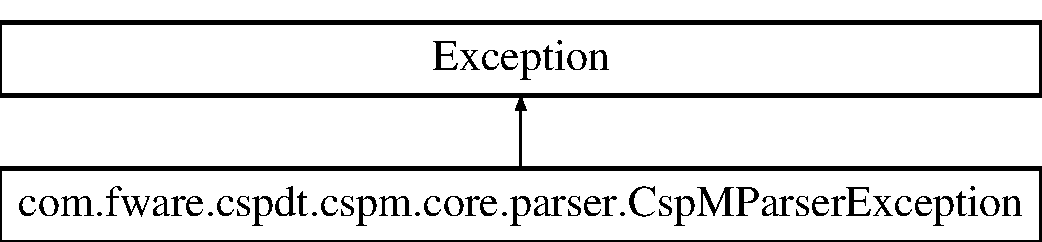
\includegraphics[height=2.000000cm]{classcom_1_1fware_1_1cspdt_1_1cspm_1_1core_1_1parser_1_1_csp_m_parser_exception}
\end{center}
\end{figure}
\subsection*{Public Member Functions}
\begin{DoxyCompactItemize}
\item 
\hyperlink{classcom_1_1fware_1_1cspdt_1_1cspm_1_1core_1_1parser_1_1_csp_m_parser_exception_af682de9d6863741515bd16984a49cba6}{Csp\+M\+Parser\+Exception} (String message, String token, int linha, int pos)
\begin{DoxyCompactList}\small\item\em Contrutor Padrao. \end{DoxyCompactList}\item 
\mbox{\Hypertarget{classcom_1_1fware_1_1cspdt_1_1cspm_1_1core_1_1parser_1_1_csp_m_parser_exception_af88518474b589e8fae93da03509406a6}\label{classcom_1_1fware_1_1cspdt_1_1cspm_1_1core_1_1parser_1_1_csp_m_parser_exception_af88518474b589e8fae93da03509406a6}} 
String {\bfseries get\+Token} ()
\item 
\mbox{\Hypertarget{classcom_1_1fware_1_1cspdt_1_1cspm_1_1core_1_1parser_1_1_csp_m_parser_exception_ab74d0acba740b8401cbe5accd59a408c}\label{classcom_1_1fware_1_1cspdt_1_1cspm_1_1core_1_1parser_1_1_csp_m_parser_exception_ab74d0acba740b8401cbe5accd59a408c}} 
int {\bfseries get\+Linha} ()
\item 
\mbox{\Hypertarget{classcom_1_1fware_1_1cspdt_1_1cspm_1_1core_1_1parser_1_1_csp_m_parser_exception_aa253986d49dda0f6bdd1a6e2646ec1ac}\label{classcom_1_1fware_1_1cspdt_1_1cspm_1_1core_1_1parser_1_1_csp_m_parser_exception_aa253986d49dda0f6bdd1a6e2646ec1ac}} 
int {\bfseries get\+Pos} ()
\end{DoxyCompactItemize}


\subsection{Detailed Description}
Excecao disparada quando a analise sintatica de um no na ast falha. 

\begin{DoxyAuthor}{Author}
A\+L\+V\+A\+RO, E\+V\+E\+R\+A\+L\+DA, F\+E\+L\+I\+PE, J\+O\+N\+A\+T\+H\+AN, J\+U\+V\+E\+N\+AL 
\end{DoxyAuthor}


\subsection{Constructor \& Destructor Documentation}
\mbox{\Hypertarget{classcom_1_1fware_1_1cspdt_1_1cspm_1_1core_1_1parser_1_1_csp_m_parser_exception_af682de9d6863741515bd16984a49cba6}\label{classcom_1_1fware_1_1cspdt_1_1cspm_1_1core_1_1parser_1_1_csp_m_parser_exception_af682de9d6863741515bd16984a49cba6}} 
\index{com\+::fware\+::cspdt\+::cspm\+::core\+::parser\+::\+Csp\+M\+Parser\+Exception@{com\+::fware\+::cspdt\+::cspm\+::core\+::parser\+::\+Csp\+M\+Parser\+Exception}!Csp\+M\+Parser\+Exception@{Csp\+M\+Parser\+Exception}}
\index{Csp\+M\+Parser\+Exception@{Csp\+M\+Parser\+Exception}!com\+::fware\+::cspdt\+::cspm\+::core\+::parser\+::\+Csp\+M\+Parser\+Exception@{com\+::fware\+::cspdt\+::cspm\+::core\+::parser\+::\+Csp\+M\+Parser\+Exception}}
\subsubsection{\texorpdfstring{Csp\+M\+Parser\+Exception()}{CspMParserException()}}
{\footnotesize\ttfamily com.\+fware.\+cspdt.\+cspm.\+core.\+parser.\+Csp\+M\+Parser\+Exception.\+Csp\+M\+Parser\+Exception (\begin{DoxyParamCaption}\item[{String}]{message,  }\item[{String}]{token,  }\item[{int}]{linha,  }\item[{int}]{pos }\end{DoxyParamCaption})\hspace{0.3cm}{\ttfamily [inline]}}



Contrutor Padrao. 


\begin{DoxyParams}{Parameters}
{\em message} & A mensagem de erro \\
\hline
{\em Token} & O token que gerou o erro \\
\hline
{\em linha} & A linha onde se encontra o token \\
\hline
{\em pos} & A coluna onde se encontra o token \\
\hline
\end{DoxyParams}


The documentation for this class was generated from the following file\+:\begin{DoxyCompactItemize}
\item 
C\+:/\+Users/\+E\+V\+A/\+Downloads/eclipse/workspace/cspdt/com.\+fware.\+cspdt.\+cspm.\+core/src/com/fware/cspdt/cspm/core/parser/Csp\+M\+Parser\+Exception.\+java\end{DoxyCompactItemize}

\hypertarget{classcom_1_1fware_1_1cspdt_1_1cspm_1_1core_1_1model_1_1_csp_m_ref}{}\section{com.\+fware.\+cspdt.\+cspm.\+core.\+model.\+Csp\+M\+Ref Class Reference}
\label{classcom_1_1fware_1_1cspdt_1_1cspm_1_1core_1_1model_1_1_csp_m_ref}\index{com.\+fware.\+cspdt.\+cspm.\+core.\+model.\+Csp\+M\+Ref@{com.\+fware.\+cspdt.\+cspm.\+core.\+model.\+Csp\+M\+Ref}}


Essa classe representa uma referencia dentro do documento C\+SP.  


\subsection*{Public Member Functions}
\begin{DoxyCompactItemize}
\item 
\hyperlink{classcom_1_1fware_1_1cspdt_1_1cspm_1_1core_1_1model_1_1_csp_m_ref_a7b1372b6ae2cfa44679cc727e6ae25b6}{Csp\+M\+Ref} (String text, int line, int pos, \hyperlink{classcom_1_1fware_1_1cspdt_1_1cspm_1_1core_1_1model_1_1_csp_m_ref}{Csp\+M\+Ref} parent)
\begin{DoxyCompactList}\small\item\em Um construtor padrao para uma referencia no documento. \end{DoxyCompactList}\item 
\mbox{\Hypertarget{classcom_1_1fware_1_1cspdt_1_1cspm_1_1core_1_1model_1_1_csp_m_ref_aaa7b66a5e3c09fb9159e2550df6e544f}\label{classcom_1_1fware_1_1cspdt_1_1cspm_1_1core_1_1model_1_1_csp_m_ref_aaa7b66a5e3c09fb9159e2550df6e544f}} 
String {\bfseries get\+Text} ()
\item 
\mbox{\Hypertarget{classcom_1_1fware_1_1cspdt_1_1cspm_1_1core_1_1model_1_1_csp_m_ref_ada5e213f20cca7a90a071cf2092521d7}\label{classcom_1_1fware_1_1cspdt_1_1cspm_1_1core_1_1model_1_1_csp_m_ref_ada5e213f20cca7a90a071cf2092521d7}} 
void {\bfseries set\+Text} (String text)
\item 
\mbox{\Hypertarget{classcom_1_1fware_1_1cspdt_1_1cspm_1_1core_1_1model_1_1_csp_m_ref_a5060a9579353dc5f230a4bbd02b571a0}\label{classcom_1_1fware_1_1cspdt_1_1cspm_1_1core_1_1model_1_1_csp_m_ref_a5060a9579353dc5f230a4bbd02b571a0}} 
int {\bfseries get\+Line} ()
\item 
\mbox{\Hypertarget{classcom_1_1fware_1_1cspdt_1_1cspm_1_1core_1_1model_1_1_csp_m_ref_ad9192aad99c6a951ebc720b3977f021c}\label{classcom_1_1fware_1_1cspdt_1_1cspm_1_1core_1_1model_1_1_csp_m_ref_ad9192aad99c6a951ebc720b3977f021c}} 
void {\bfseries set\+Line} (int line)
\item 
\mbox{\Hypertarget{classcom_1_1fware_1_1cspdt_1_1cspm_1_1core_1_1model_1_1_csp_m_ref_a0af743b98ab418c11987b2338581f316}\label{classcom_1_1fware_1_1cspdt_1_1cspm_1_1core_1_1model_1_1_csp_m_ref_a0af743b98ab418c11987b2338581f316}} 
int {\bfseries get\+Pos} ()
\item 
\mbox{\Hypertarget{classcom_1_1fware_1_1cspdt_1_1cspm_1_1core_1_1model_1_1_csp_m_ref_a76a816233b105e1732ebbb96372c798c}\label{classcom_1_1fware_1_1cspdt_1_1cspm_1_1core_1_1model_1_1_csp_m_ref_a76a816233b105e1732ebbb96372c798c}} 
void {\bfseries set\+Pos} (int pos)
\item 
\mbox{\Hypertarget{classcom_1_1fware_1_1cspdt_1_1cspm_1_1core_1_1model_1_1_csp_m_ref_af92897900ebe2e750ff4c2c3ff22e696}\label{classcom_1_1fware_1_1cspdt_1_1cspm_1_1core_1_1model_1_1_csp_m_ref_af92897900ebe2e750ff4c2c3ff22e696}} 
\hyperlink{classcom_1_1fware_1_1cspdt_1_1cspm_1_1core_1_1model_1_1_csp_m_ref}{Csp\+M\+Ref} {\bfseries get\+Parent} ()
\item 
\mbox{\Hypertarget{classcom_1_1fware_1_1cspdt_1_1cspm_1_1core_1_1model_1_1_csp_m_ref_a46a58dfea317d1e36490608110b1ddc7}\label{classcom_1_1fware_1_1cspdt_1_1cspm_1_1core_1_1model_1_1_csp_m_ref_a46a58dfea317d1e36490608110b1ddc7}} 
void {\bfseries set\+Parent} (\hyperlink{classcom_1_1fware_1_1cspdt_1_1cspm_1_1core_1_1model_1_1_csp_m_ref}{Csp\+M\+Ref} parent)
\end{DoxyCompactItemize}


\subsection{Detailed Description}
Essa classe representa uma referencia dentro do documento C\+SP. 

Essa classe mostra o spelling de um token e a linha e coluna em que ele se encontra. Tambem traz uma referencia ao seu elemento pai na hierarquia da A\+ST.

\begin{DoxyAuthor}{Author}
A\+L\+V\+A\+RO, E\+V\+E\+R\+A\+L\+DA, F\+E\+L\+I\+PE, J\+O\+N\+A\+T\+H\+AN, J\+U\+V\+E\+N\+AL 
\end{DoxyAuthor}


\subsection{Constructor \& Destructor Documentation}
\mbox{\Hypertarget{classcom_1_1fware_1_1cspdt_1_1cspm_1_1core_1_1model_1_1_csp_m_ref_a7b1372b6ae2cfa44679cc727e6ae25b6}\label{classcom_1_1fware_1_1cspdt_1_1cspm_1_1core_1_1model_1_1_csp_m_ref_a7b1372b6ae2cfa44679cc727e6ae25b6}} 
\index{com\+::fware\+::cspdt\+::cspm\+::core\+::model\+::\+Csp\+M\+Ref@{com\+::fware\+::cspdt\+::cspm\+::core\+::model\+::\+Csp\+M\+Ref}!Csp\+M\+Ref@{Csp\+M\+Ref}}
\index{Csp\+M\+Ref@{Csp\+M\+Ref}!com\+::fware\+::cspdt\+::cspm\+::core\+::model\+::\+Csp\+M\+Ref@{com\+::fware\+::cspdt\+::cspm\+::core\+::model\+::\+Csp\+M\+Ref}}
\subsubsection{\texorpdfstring{Csp\+M\+Ref()}{CspMRef()}}
{\footnotesize\ttfamily com.\+fware.\+cspdt.\+cspm.\+core.\+model.\+Csp\+M\+Ref.\+Csp\+M\+Ref (\begin{DoxyParamCaption}\item[{String}]{text,  }\item[{int}]{line,  }\item[{int}]{pos,  }\item[{\hyperlink{classcom_1_1fware_1_1cspdt_1_1cspm_1_1core_1_1model_1_1_csp_m_ref}{Csp\+M\+Ref}}]{parent }\end{DoxyParamCaption})\hspace{0.3cm}{\ttfamily [inline]}}



Um construtor padrao para uma referencia no documento. 


\begin{DoxyParams}{Parameters}
{\em text} & O spelling do token sendo referenciado \\
\hline
{\em line} & A linha em que se encontra \\
\hline
{\em pos} & A coluna em que esta (posicao dentro da linha) \\
\hline
{\em parent} & O elemento pai na A\+ST \\
\hline
\end{DoxyParams}


The documentation for this class was generated from the following file\+:\begin{DoxyCompactItemize}
\item 
C\+:/\+Users/\+E\+V\+A/\+Downloads/eclipse/workspace/cspdt/com.\+fware.\+cspdt.\+cspm.\+core/src/com/fware/cspdt/cspm/core/model/Csp\+M\+Ref.\+java\end{DoxyCompactItemize}

\hypertarget{classcom_1_1fware_1_1cspdt_1_1cspm_1_1core_1_1model_1_1_token_extractor}{}\section{com.\+fware.\+cspdt.\+cspm.\+core.\+model.\+Token\+Extractor Class Reference}
\label{classcom_1_1fware_1_1cspdt_1_1cspm_1_1core_1_1model_1_1_token_extractor}\index{com.\+fware.\+cspdt.\+cspm.\+core.\+model.\+Token\+Extractor@{com.\+fware.\+cspdt.\+cspm.\+core.\+model.\+Token\+Extractor}}


Classe que extrai tokens da ast.  


Inheritance diagram for com.\+fware.\+cspdt.\+cspm.\+core.\+model.\+Token\+Extractor\+:\begin{figure}[H]
\begin{center}
\leavevmode
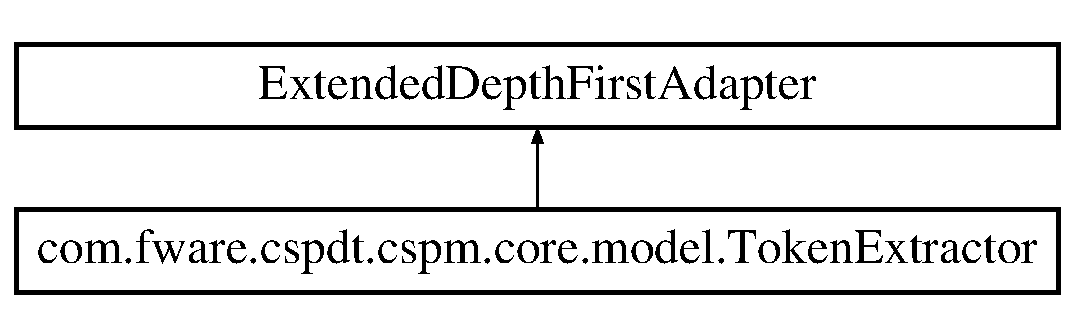
\includegraphics[height=2.000000cm]{classcom_1_1fware_1_1cspdt_1_1cspm_1_1core_1_1model_1_1_token_extractor}
\end{center}
\end{figure}
\subsection*{Public Member Functions}
\begin{DoxyCompactItemize}
\item 
\mbox{\Hypertarget{classcom_1_1fware_1_1cspdt_1_1cspm_1_1core_1_1model_1_1_token_extractor_a263d3c54e093019448fce4a8a8a7bd1f}\label{classcom_1_1fware_1_1cspdt_1_1cspm_1_1core_1_1model_1_1_token_extractor_a263d3c54e093019448fce4a8a8a7bd1f}} 
Token {\bfseries get\+First\+Token} ()
\item 
\mbox{\Hypertarget{classcom_1_1fware_1_1cspdt_1_1cspm_1_1core_1_1model_1_1_token_extractor_ab9ccc78cbbe7c3d1fc54f7bdd8301572}\label{classcom_1_1fware_1_1cspdt_1_1cspm_1_1core_1_1model_1_1_token_extractor_ab9ccc78cbbe7c3d1fc54f7bdd8301572}} 
Token {\bfseries get\+Last\+Token} ()
\item 
\mbox{\Hypertarget{classcom_1_1fware_1_1cspdt_1_1cspm_1_1core_1_1model_1_1_token_extractor_a760a9a62e1352ccda5e0bf35feeb86f9}\label{classcom_1_1fware_1_1cspdt_1_1cspm_1_1core_1_1model_1_1_token_extractor_a760a9a62e1352ccda5e0bf35feeb86f9}} 
void {\bfseries default\+In} (Node node)
\end{DoxyCompactItemize}


\subsection{Detailed Description}
Classe que extrai tokens da ast. 

The documentation for this class was generated from the following file\+:\begin{DoxyCompactItemize}
\item 
C\+:/\+Users/\+E\+V\+A/\+Downloads/eclipse/workspace/cspdt/com.\+fware.\+cspdt.\+cspm.\+core/src/com/fware/cspdt/cspm/core/model/Token\+Extractor.\+java\end{DoxyCompactItemize}

%--- End generated contents ---

% Index
\backmatter
\newpage
\phantomsection
\clearemptydoublepage
\addcontentsline{toc}{chapter}{Index}
\printindex

\end{document}
